\documentclass{article}
\usepackage[preprint,nonatbib]{neurips_2025}
\usepackage[T1]{fontenc}
\usepackage{microtype}
\usepackage{amsmath,amssymb}
\usepackage{booktabs}
\usepackage{graphicx}
\usepackage[hidelinks]{hyperref}
\makeatletter
\renewcommand{\@noticestring}{CIS 6220 final-project draft. November 2026.}
\makeatother
\title{Agentic Scene Reconstruction:\\Small Objects, Execution Efficiency, and Cost}
\author{Yifan Hu \qquad Mingjian Li \qquad Yujing Li\\University of Pennsylvania\\CIS 6220: Deep Learning at Scale}
\begin{document}
\maketitle
\begin{abstract}
AHa-3D gives an agent tools to reconstruct a room, but the agent must decide
which objects to build and how long to keep repairing them. On one AI2-THOR
room, it produced eight scene versions and correctly placed 7 of 34 objects
by box overlap after scale alignment. We study two ways to coordinate
object-level work. AHA-driven gives the agent a detector inventory, independent
build tasks and a repair limit. It placed 16 objects correctly, but its
supervisor alone cost an estimated \$28.88 in tokens, exceeding the original
run's \$27.27. AHA-auto moves scheduling and retry decisions into Python.
With the same model in both controllers, auto placed 11 objects correctly
for \$10.78, compared with driven's \$38.55. Both placed five of the 12
objects measuring 20 to under 50\,cm by fitted-scale overlap, up from one
for the baseline. In a separate study across three CA-1M rooms, expanding
the task to all visible objects and supplying detector evidence raised
center-and-size recall in that size range from 2 to 30 of 174.
\end{abstract}

\begin{figure}[t]
\centering
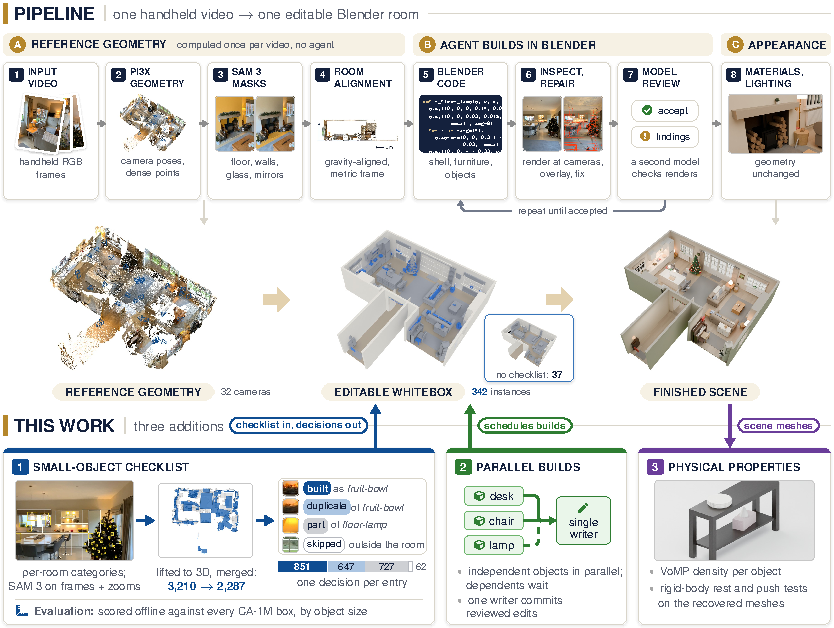
\includegraphics[width=\linewidth]{figures/system-pipeline.pdf}
\caption{\textbf{System overview.} Top: AHa-3D~\cite{aha3d} computes a
reference geometry from a handheld video, an agent authors the room in
Blender against renders from the video's cameras, and an optional pass adds
materials. Middle: one held-out room at each stage; instances under 50\,cm
are blue, and the inset is the same room built without the checklist.
Bottom: our additions, a detector checklist for small objects
(Section~\ref{sec:small-method}; the four entries are real, and the bar
counts the agent's decisions on all 2{,}287 entries of six held-out rooms),
concurrent object builds (Section~\ref{sec:architecture}) and physical
properties (Section~\ref{sec:physics-plan}).}
\label{fig:system}
\end{figure}


\section{Introduction}
Picking up a cushion requires a scene in which it can move independently of
the sofa. In an AHa-3D reconstruction of an AI2-THOR living room~\cite{aha3d,ai2thor},
only one of 18 annotated objects under 50\,cm was correctly placed as a separate
instance. Giving existing parts, including a sofa cushion, their own identities
raised that count to four without moving any geometry. Objects on a dressing
table or windowsill illustrate the problem in real rooms (Figure~\ref{fig:scope}).

\textbf{Who decides when to try again?}
Original AHa-3D provides an indoor-scene workflow as a skill for a coding
agent. On FloorPlan209 the agent overlapped preview rendering with review,
but built the furniture sequentially in a shared Blender scene. Its trace
records eight room-scene versions and nine build
commands, including an interrupted first build and its rerun. Five attempts
to prepare layout evidence included two failures due to missing views.
After 42 minutes the candidate still failed review. The trace records
room-level revisions, leaving the cost of retrying any one object unknown.

We ask whether explicit object identities, dependencies and repair limits
can improve small-object coverage while reducing the cost of repeated work.
AHA-driven keeps an agent in charge of these decisions. Profiling its
supervisor shows how much inference it spends waiting for workers.
AHA-auto lets a model plan the room, then gives those execution decisions
to Python. We compare their costs and placements on FloorPlan209
(Section~\ref{sec:parallel-time}). Separately, on three CA-1M rooms~\cite{ca1m},
we vary object instructions, detector evidence and mesh generation to test
which changes improve placement (Section~\ref{sec:existing-reconstruction}).

\section{Related Work}
\textbf{From scans to editable objects.}
Scan2CAD aligns CAD models to partial RGB-D geometry~\cite{scan2cad}.
LiteReality retrieves assets and transfers appearance from indoor scans~\cite{litereality}.
A well-aligned table can still be missing its plates. We use CA-1M's annotated boxes~\cite{ca1m} to measure
instance placement, then examine the role of mesh volume in a separate
rigid-body pilot using VoMP's predicted density~\cite{vomp}.

\textbf{Scene authoring and inverse graphics.}
SceneSmith uses agents to furnish rooms from text, down to clutter on individual
surfaces~\cite{scenesmith}. Recovering a particular room requires each object to
correspond to an observation. VIGA uses the discrepancy between a render and its
target to guide the next code edit~\cite{viga}. LEGO-Anything revises Blender code
against one image and scores visible geometry separately from whether the program runs~\cite{legoanything}.
SceneConductor delegates local repairs to specialists after inferring a layout
from one image~\cite{sceneconductor}. With metric RGB-D input, LiteReality-Agent
edits a persistent room program, compares rendered and captured views, and checks
support and collisions~\cite{literealityagent}. Our input is RGB video. After aligning camera
trajectories for scoring, we measure placement recall by object size, counting
targets that the agent never attempted.

\textbf{Where to spend inference.}
Fast-SAM3D accelerates single-view asset generation by caching intermediate
computation and reducing redundant tokens~\cite{fastsam3d}. At the workflow level,
LLMCompiler schedules independent tool calls in parallel~\cite{llmcompiler}, and
FrugalGPT routes queries through a model cascade~\cite{frugalgpt}. Workers editing a room share
state. They can build meshes concurrently, but raising a shelf changes the required
height of every object on it. Our controllers track these dependencies and verify
each change against the current scene.

\section{Methods}
\subsection{Reconstructing and evaluating small objects}
\label{sec:small-method}
We study how instance-level instructions and a visual inventory affect
small-object reconstruction in AHa-3D (Figure~\ref{fig:system}, bottom left).
A \emph{target} is an annotated CA-1M box, and an \emph{instance} is a
set of reconstructed mesh parts with a common identifier.

\textbf{All objects} switches AHa-3D from its major-object setting to its
all-object setting (\texttt{precise}). The prompt requires a distinct
identifier for each visible item so that it can move independently of its support.

\begin{figure}[t]
\centering
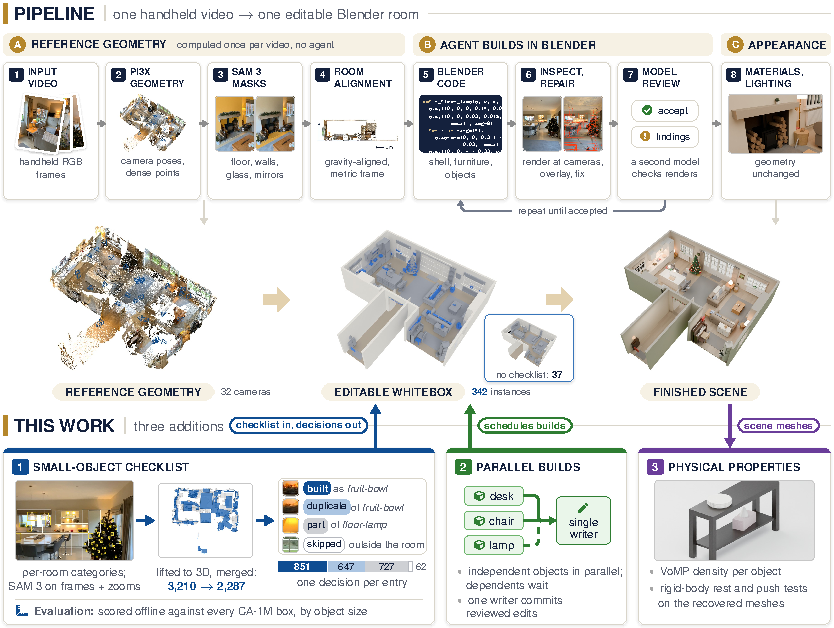
\includegraphics[width=\linewidth]{figures/system-pipeline.pdf}
\caption{\textbf{System overview.} Top: AHa-3D~\cite{aha3d} computes a
reference geometry from a handheld video, an agent authors the room in
Blender against renders from the video's cameras, and an optional pass adds
materials. Middle: one held-out room at each stage; instances under 50\,cm
are blue, and the inset is the same room built without the checklist.
Bottom: our additions, a detector checklist for small objects
(Section~\ref{sec:small-method}; the four entries are real, and the bar
counts the agent's decisions on all 2{,}287 entries of six held-out rooms),
concurrent object builds (Section~\ref{sec:architecture}) and physical
properties (Section~\ref{sec:physics-plan}).}
\label{fig:system}
\end{figure}

\textbf{Inventory} pairs Boxer's predicted 3D boxes and categories~\cite{boxer}
with crops from the video. The agent builds each listed item or explains an
omission, and can still build items Boxer missed. Two further variants let
this agent call an image-to-mesh model,
\href{https://huggingface.co/tencent/Hunyuan3D-2mini}{Hunyuan3D-2mini}~\cite{hunyuan3d2}, for
every object under 50\,cm (\textbf{Required generation}) or at its own
discretion (\textbf{Selective generation}); a generated mesh that fails a
check of silhouette, 3D points, dimensions and support is replaced by
primitives.

\textbf{Revised inventory.}
To improve coverage below 20\,cm, we adapt SceneRig's detection
stage~\cite{scenerig}. A language model extends a fixed category list
with categories observed in eight frames. SAM~3~\cite{sam3} segments them in
full-resolution frames and in nine overlapping zoomed windows, keeping
window-only detections that appear in at least two frames. MoGe-2
depth~\cite{moge2}, rescaled to the reference geometry, lifts each mask to a
3D box. Boxes are then moved onto the surface below them, and similar boxes
of one category share a size.

\textbf{Checklist} uses the revised inventory. We merge same-category
entries when their 3D intersection over union (IoU) exceeds 0.4 or their
centers lie within one fifth of the shorter box diagonal. Across the six
held-out rooms, this reduces 3{,}210 entries to 2{,}287 (Boxer yields 364).
To account for redundant detections, the agent labels each entry as
\emph{built} (a separate instance), \emph{duplicate} (an existing instance),
\emph{part} (of a larger object), or \emph{skipped}. The prompt requires
separate instances for individual objects in stacks or rows. We fixed the
thresholds and prompt on development rooms before held-out evaluation.

\textbf{Camera alignment.}
Each instance is scored as one upright box enclosing its mesh parts. Monocular
video leaves room scale and heading uncertain. For reconstructed and annotated
camera centers $x_i$ and $y_i$ at corresponding frames, the room transform is
\begin{equation}
 T(x)=sR_z(\theta)x+t,\qquad
 (\hat{s},\hat{\theta},\hat{t})=
 \arg\min_{s,\theta,t}\sum_i \lVert T(x_i)-y_i\rVert_2^2 .
 \label{eq:camera-alignment}
\end{equation}
Here $R_z$ rotates about the vertical axis. Object annotations enter only
during offline scoring.

\textbf{Matching and outcomes.}
For an aligned prediction $P$ and target $G$, let $d$ be their center distance,
$L$ the full diagonal of $G$, and $r$ the predicted longest side divided by the
target's longest side. A candidate pair must satisfy $1/3\le r\le 3$ and either
$d\le\max(L/2,0.30\,\mathrm{m})$ or a 3D IoU of at least 0.10.
We greedily match pairs in ascending order of $2d/L+|\log r|$, using
each box at most once regardless of category. A
matched target is \emph{correctly placed} if
\begin{equation}
 d\le\max(0.10\,\mathrm{m},L/4)\quad\text{and}\quad 0.67\le r\le 1.5,
 \label{eq:center-size}
\end{equation}
and \emph{misplaced} otherwise; an unmatched target has no reconstruction.
The three outcomes separate a coverage failure from a placement failure. We
report them by the target's longest side: under 20\,cm, 20 to under 50\,cm,
50\,cm to under 1.5\,m, and larger. Reconstructed instances that match no
target carry no penalty and are reported separately.
Appendix~\ref{app:small} adds a box-overlap criterion and a fit without
scale.

\subsection{Scheduling object construction}
\label{sec:architecture}
Reconstructing more objects creates more opportunities to work in parallel.
Two workers can build a desk and a chair independently. A third worker placing
a lamp on the desk needs its final height. We implement two controllers for
AHa-3D that use these dependencies while retaining its camera estimates,
geometry tools and scene review (Figure~\ref{fig:blueprint}).

\begin{figure}[!htbp]
\centering
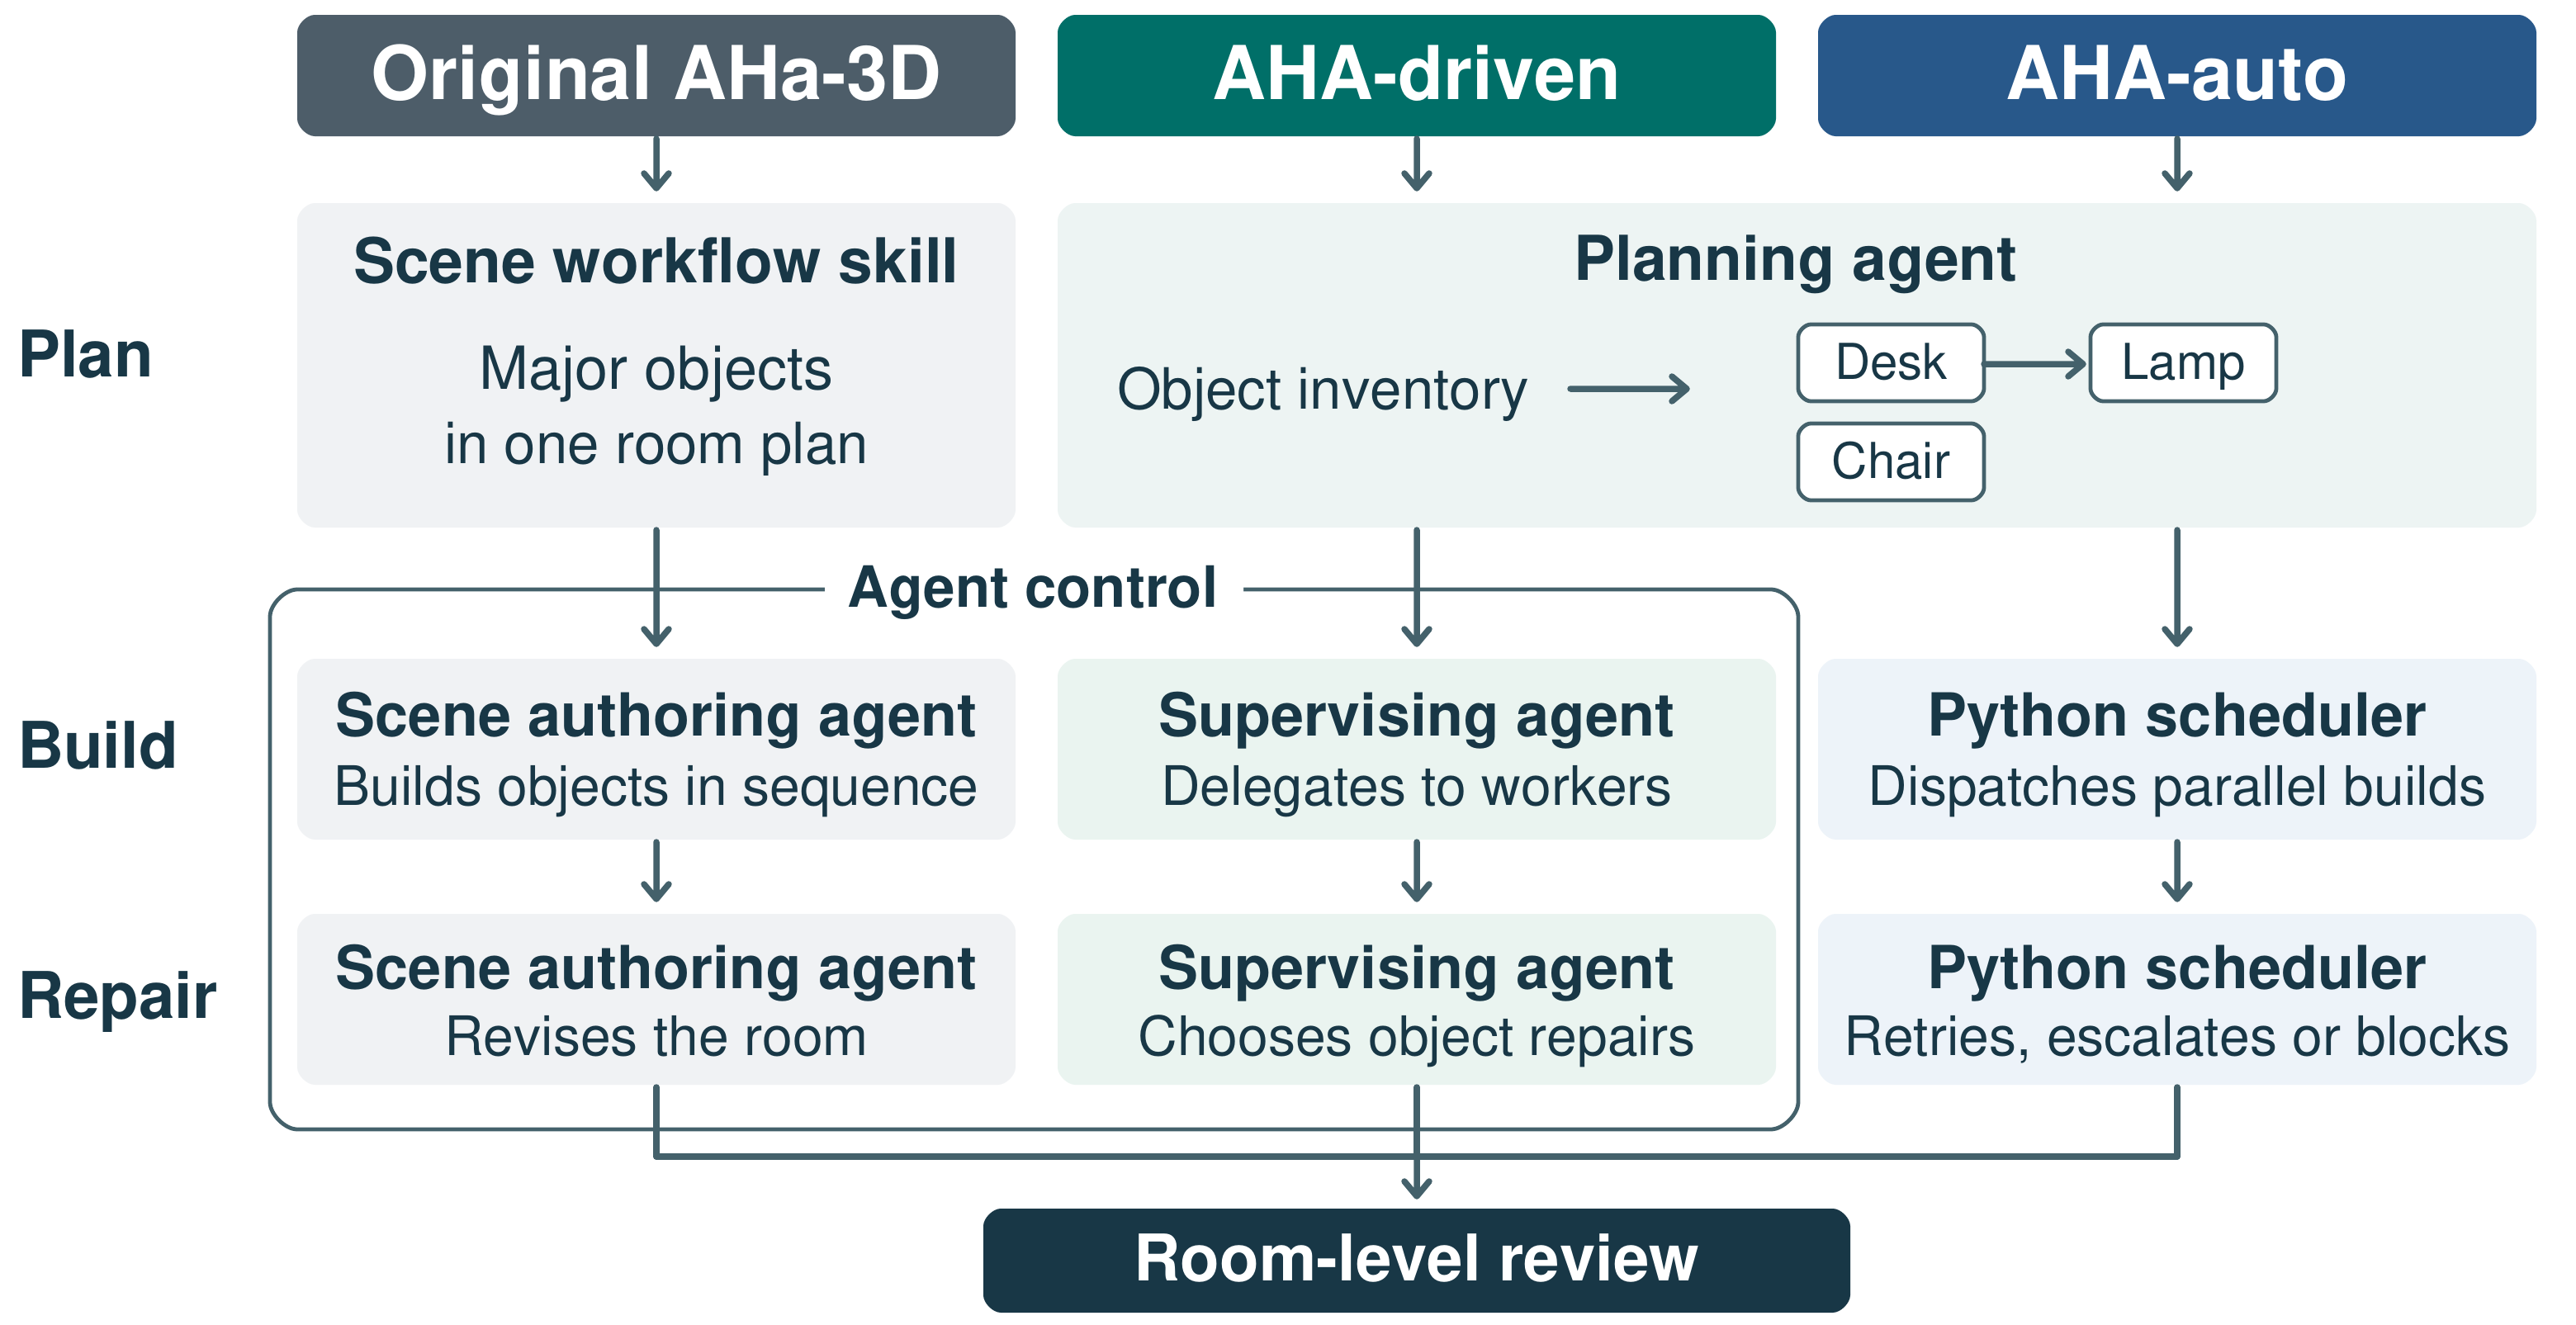
\includegraphics[width=\linewidth]{figures/parallelism.png}
\caption{The desk and chair can be built from the same scene. The lamp waits
for the desk to be committed. Workers build isolated candidates, and a single
writer incorporates reviewed edits into the shared room.}
\label{fig:blueprint}
\end{figure}

In \textbf{AHA-auto}, a model plans the tasks and a program dispatches ready
work, retries failed builds and escalates difficult cases to a stronger model.
In \textbf{AHA-agent-driven}, a supervisor chooses which tasks to delegate,
when to review them and how to repair a failed edit. Both controllers allow
tasks to run together only after their prerequisites are complete and when
neither task changes objects the other uses.

Workers edit separate scene copies. Before an edit becomes part of the room,
the controller checks the saved geometry and cameras, verifies that unrelated
objects were preserved and reviews the proposed change against the current
scene. A short Blender benchmark and available memory limit the number of
simultaneous builds. GPU generation and writes to the shared scene run serially.


\subsection{Accounting for time and cost}
Parallel workers can shorten elapsed time while making the same number of model
calls. We measure elapsed time from the start of a reconstruction to its end.
For cost, we add the charges for input, cached input and output tokens to the
cost of the compute used by the run. Overlapping jobs on one billed host incur
one host charge for the shared interval. Failed calls, repairs and reviews
also consume resources. To compare workflows at the same acceptance standard,
we divide the total cost of all attempts by the number of accepted rooms.

\section{Physical properties of recovered objects}
\label{sec:physics-plan}
A plate can occupy the correct 3D box yet move unrealistically when pushed.
We test this distinction on a coffee table reconstructed by Inventory.
For each plate and the tissue-box assembly, we divide the mesh into volume
cells and estimate density with pretrained VoMP~\cite{vomp}. Each cell
contributes its density times its volume to the object's mass. The distribution
of that mass determines the center of mass and resistance to rotation.
We compare a uniform density, VoMP's object-average density and its spatially
varying density while holding the geometry fixed. We set friction separately
so we can test its effect on the same objects.


\section{Experiments}
\subsection{Datasets and experimental design}
\textbf{Small-object reconstruction on CA-1M.} We use handheld RGB video
from three held-out rooms to test how object instructions, detector evidence
and mesh generation affect placement (Figure~\ref{fig:settings}).
The five variants share a reconstruction model, reference geometry and seed.
We score all 15 outputs against 513 annotated targets, including 174 measuring
20 to under 50\,cm~\cite{ca1m}. One room supplies the recovered objects for
the physics pilot. Figure~\ref{fig:scope} uses separate development rooms.
Boxer was trained in part on the CA-1M training set~\cite{boxer}.

\textbf{Controller evaluation in AI2-THOR.} We use one simulated living room,
FloorPlan209~\cite{ai2thor}, to trace failures in original AHa-3D and compare
its placement recall and token cost with AHA-driven and AHA-auto on the same
34 targets. A separate four-object Blender benchmark uses the room shell
and a fixed model delay to measure the effect of parallel scheduling.

\begin{figure}[!htbp]
\centering
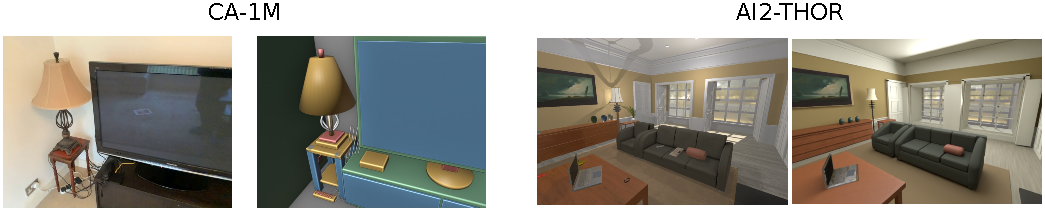
\includegraphics[width=\linewidth]{figures/experimental-settings.pdf}
\caption{Input and reconstruction in each setting. CA-1M shows the All
objects variant on a held-out living room. AI2-THOR shows original AHa-3D
on the room used to compare controllers.}
\label{fig:settings}
\end{figure}

\subsection{Small-object coverage and placement}
\label{sec:existing-reconstruction}
Across the first three held-out rooms, Inventory correctly placed \textbf{30 of 174}
small objects by center and size, compared with \textbf{2 of 174} for original
AHa-3D and 25 for All objects (Table~\ref{tab:small-placement}). With box
overlap as the criterion, the count rose from two to 20 to 21.

\begin{table}[!htbp]
\centering\small
\caption{Small objects correctly placed out of 174 in three held-out rooms.
All objects expands the baseline scope. Inventory adds detector evidence.
The last two rows use the same generator, triggered by object size or by the agent. Parentheses
give gains over the baseline with scale fitted from cameras.}
\label{tab:small-placement}
\begin{tabular}{lrrrr}
\toprule
& \multicolumn{2}{c}{Fitted scale} & \multicolumn{2}{c}{Fixed scale} \\
\cmidrule(lr){2-3}\cmidrule(lr){4-5}
Variant & Center and size & Box overlap & Center and size & Box overlap \\
\midrule
AHa-3D (baseline) & 2 & 2 & 2 & 1 \\
All objects & 25 (+23) & 20 (+18) & 12 & 7 \\
Inventory & \textbf{30 (+28)} & \textbf{21 (+19)} & 13 & 7 \\
\midrule
Required generation & 24 (+22) & 21 (+19) & 9 & 7 \\
Selective generation & 26 (+24) & 18 (+16) & 10 & 6 \\
\bottomrule
\end{tabular}
\end{table}

Relative to All objects, Inventory's net gain was five placements by center
and size, one by fitted-scale overlap and zero by fixed-scale overlap.
Below 20\,cm, Boxer's inventory loosely matched only 10 of the 138 targets
in these rooms, and the Inventory reconstruction correctly placed nine.

Neither generation policy improved on Inventory's 30 small-object placements
by center and size. Across both policies, 160 generation attempts yielded ten
accepted placements and five generated assets in the saved scenes. Flat meshes,
incorrect dimensions and poor silhouette fits prompted the agent to fall back
to procedural geometry.

\textbf{Six rooms and the checklist.}
We then ran the baseline, All objects, Inventory and Checklist on three
further held-out rooms, the next in a fixed order, and ran Checklist on the
first three. The six rooms hold 857 targets: 264 under 20\,cm and 279 from
20 to under 50\,cm (Table~\ref{tab:outcomes}). Of these 543 targets under
50\,cm, the baseline correctly placed 6, All objects 71, Inventory 101 and
Checklist 142. Checklist left 257 of them without a matched reconstruction,
against 361 for Inventory.

\begin{table}[!htbp]
\centering\small
\caption{Outcome of each of the 857 targets in six held-out rooms under the
center-and-size test with fitted scale. Each cell gives targets correctly
placed / matched but misplaced / left without a matched reconstruction.}
\label{tab:outcomes}
\begin{tabular}{lcccc}
\toprule
Variant & $<$20\,cm (264) & 20--$<$50\,cm (279) & 50--$<$150\,cm (206) & $\ge$150\,cm (108) \\
\midrule
AHa-3D (baseline) & 0 / 0 / 264 & 6 / 6 / 267 & 47 / 5 / 154 & 30 / 4 / 74 \\
All objects & 21 / 26 / 217 & 50 / 55 / 174 & 82 / 23 / 101 & 45 / 8 / 55 \\
Inventory & 36 / 22 / 206 & 65 / 59 / 155 & 93 / 22 / 91 & 43 / 11 / 54 \\
Checklist & \textbf{50} / 65 / 149 & \textbf{92} / 79 / 108 & 92 / 31 / 83 & \textbf{50} / 12 / 46 \\
\bottomrule
\end{tabular}
\end{table}

Table~\ref{tab:paired} compares variants room by room. All objects beat the
baseline in all six rooms, the strongest result six rooms can give. Checklist
gained 71 placements over All objects, 41 of them in the room with a wall of
postcards, and was ahead of Inventory in three rooms and behind in three.
Neither difference is significant. Moving every reconstructed instance by a
random 0.5 to 1.5\,m left Checklist with about four correct placements under
50\,cm, so the gain is not an effect of building more boxes. Checklist runs
averaged 79 minutes and \$13.28, against 59 minutes and \$12.36 for All
objects and 104 minutes and \$19.95 for Inventory.

\begin{table}[!htbp]
\centering\small
\caption{Difference in targets under 50\,cm correctly placed in each
held-out room. $p$: exact two-sided sign-flip test over rooms; with six
rooms it cannot fall below 0.031.}
\label{tab:paired}
\begin{tabular}{lrrrrrrr}
\toprule
Room (targets) & 1 (38) & 2 (258) & 3 (16) & 4 (71) & 5 (32) & 6 (128) & Total \\
\midrule
All objects $-$ baseline & $+8$ & $+15$ & $+7$ & $+7$ & $+8$ & $+20$ & $+65$ ($p=0.031$) \\
Inventory $-$ All objects & $-1$ & $+7$ & $+1$ & $+7$ & $+2$ & $+14$ & $+30$ ($p=0.094$) \\
Checklist $-$ All objects & $+9$ & $+18$ & $-3$ & $+5$ & $+1$ & $+41$ & $+71$ ($p=0.094$) \\
Checklist $-$ Inventory & $+10$ & $+11$ & $-4$ & $-2$ & $-1$ & $+27$ & $+41$ ($p=0.25$) \\
\bottomrule
\end{tabular}
\end{table}

The agent recorded a decision for all 2{,}287 checklist entries: 851 built,
647 duplicates, 727 parts of larger objects and 62 skipped. Checklist matched
more targets under 50\,cm than Inventory, 286 against 182, but half of its matches
failed the center-and-size test, so placement now limits it as much as
coverage. One Checklist run in room 2 ended without external review when
the reviewer's quota ran out; we repeated it, and the excluded run placed 36
targets under 50\,cm against 33 for the repeat.

Recall ignores reconstructed instances that match no target. In the first
three rooms these were 39 of 208 for All objects and 24 of 198 for
Inventory. One author checked all 63 against the video: 22 were present
where reconstructed but not annotated, 27 were real but too far off to
match, five were repeats and nine did not appear.
Checklist built 922 instances in six rooms, and 451 matched no target: 168
are postcards on one wall and 108 ornaments on one Christmas tree, which
CA-1M does not annotate one by one. The rest are unchecked.

\textbf{A revised inventory on development rooms.}
Table~\ref{tab:inventory} scores inventories on their own in five development
rooms, treating each inventory box as a placed object. Boxer's boxes passed
center and size for 10\% of the 216 targets under 20\,cm, and SAM~3 with a
fixed category list for 13\%. Room-specific categories raised this to 61\%.
The complete revised inventory reached 58\%, and 51\% of the 141 small
targets. With every box shifted horizontally by a random 0.5 to 1.5\,m
before the final step, about 1\% passed.

\begin{table}[!htbp]
\centering\small
\caption{Inventories scored without an agent on five development rooms.
Rows beginning with + add one step to the row above. Matched: share of
targets with a candidate match. Placed: share whose inventory box passes
center and size. Entries matched: share of inventory entries that match any
target.}
\label{tab:inventory}
\begin{tabular}{lrrrrrr}
\toprule
& & Entries & \multicolumn{2}{c}{$<$20\,cm (216)} & \multicolumn{2}{c}{20--$<$50\,cm (141)} \\
\cmidrule(lr){4-5}\cmidrule(lr){6-7}
Inventory & Entries & matched & Matched & Placed & Matched & Placed \\
\midrule
Boxer & 334 & 66\% & 16\% & 10\% & 57\% & 38\% \\
SAM~3, fixed categories & 745 & 34\% & 27\% & 13\% & 69\% & 39\% \\
+ windows, room categories & 2{,}123 & 20\% & 82\% & 61\% & 81\% & 50\% \\
+ MoGe-2 depth & 2{,}295 & 19\% & 81\% & 58\% & 79\% & 55\% \\
+ support and shared size & 2{,}295 & 19\% & 81\% & 58\% & 79\% & 51\% \\
\bottomrule
\end{tabular}
\end{table}

Two cautions apply. The revised inventory lists 2{,}295 entries against
745, and the share that match a target fell from 34\% to 19\%: it contains
duplicates and object parts. One refrigerator door covered with magnets and
photographs holds 112 of the 216 smallest targets; without that room, the
gain is from 18\% to 40\%. On the six held-out rooms, scored after the
Checklist settings were fixed, the revised inventory placed 32\% of targets
under 20\,cm and 41\% of small targets, against 6\% and 25\% for Boxer.

\subsection{Parallel build time and controller efficiency}
\label{sec:parallel-time}
\textbf{Controlled parallel builds.} Building the same four objects with four
Blender workers reduced elapsed time from 11.32 to 6.63 seconds
(41\%, or $1.71\times$ speedup). Both conditions used four deterministic
model responses with a two-second delay per build and scripted visual reviews.
Both committed all four objects and preserved the existing objects and cameras.
Parallel execution overlapped independent builds, while edits to the shared
scene remained serial.

\textbf{Placement on FloorPlan209.} AHA-driven-short achieved the highest
placement counts under all four criteria (Table~\ref{tab:auto-floorplan209}).
At fitted scale, it correctly placed 16 of 34 targets by box overlap,
compared with seven for original AHa-3D (Figure~\ref{fig:settings}, right).
Among the 12 targets from 20 to under 50\,cm, correct placements rose from
one to five by overlap and from one to six by center and size. All four runs
missed the six targets under 20\,cm by overlap. The driven and auto runs
used the same prepared reference, 37 Boxer detections and crops, and GPT-6
Astra at medium reasoning effort. We scored each exported scene using its
authored instance groups.

\begin{table}[!htbp]
\centering\small
\caption{FloorPlan209. Placement counts use 34 targets and alignment to 32
camera positions. Fitted scale allows uniform rescaling. Fixed scale preserves
authored size. Time covers the original session through handoff, the driven
sessions from initialization to report, and the auto construction run.}
\label{tab:auto-floorplan209}
\setlength{\tabcolsep}{3pt}
\begin{tabular}{@{}lrrrr@{}}
\toprule
Measure & Original AHa-3D & AHA-driven-short & AHA-driven-long & AHA-auto \\
\midrule
Box overlap, fitted scale & 7 & \textbf{16} & 10 & 11 \\
Box overlap, fixed scale & 6 & \textbf{9} & 6 & 4 \\
Center and size, fitted scale & 8 & \textbf{20} & 11 & 13 \\
Center and size, fixed scale & 8 & \textbf{14} & 9 & 7 \\
\midrule
Recorded time (min) & 42.1 & 49.8 & 30.1 & 30.2 \\
Cached input tokens & 17,673,472 & 27,124,992 & 10,356,352 & 783,872 \\
Uncached input tokens & 557,515 & 759,533 & 591,371 & 742,829 \\
Output tokens & 80,492 & 76,564 & 76,693 & 51,434 \\
Total recorded tokens & 18,311,479 & 27,961,089 & 11,024,416 & 1,578,135 \\
Estimated token cost (USD) & 27.27 & 38.55 & 20.10 & \textbf{10.78} \\
\bottomrule
\end{tabular}
\end{table}

\begin{figure}[!htbp]
\centering
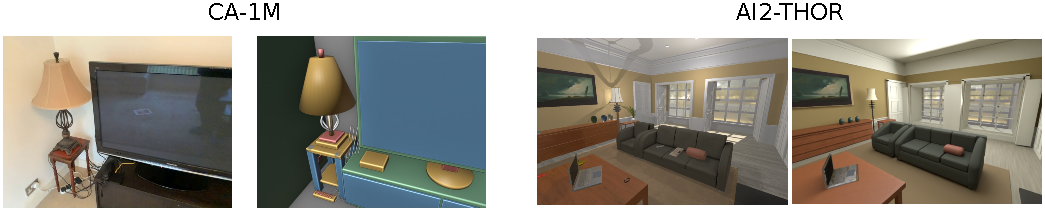
\includegraphics[width=\linewidth]{figures/experimental-settings.pdf}
\caption{Input and reconstruction in each setting. CA-1M shows the All
objects variant on a held-out living room. AI2-THOR shows original AHa-3D
on the room used to compare controllers.}
\label{fig:settings}
\end{figure}

\textbf{Cost of checking worker progress.} While Blender workers built
objects, the supervisor repeatedly checked whether they had finished, and each
call processed the conversation history again (mean context 121k tokens).
In the short-wait run, 149 of the supervisor's 216 calls only slept or polled
a running command; they used 71\% of its input tokens and an estimated
\$19.78 of the run's \$38.55 (Appendix~\ref{app:tokens}). The long-wait run
used 118 supervisor calls and cost \$20.10. Its savings came almost entirely
from cached input (\$27.12 to \$10.36), while uncached input and output
changed little. It also reused the existing plan and completed four of six
tasks, so the savings cannot be attributed to waiting alone.

\textbf{Cost and placement under Python scheduling.} AHA-auto cost \$10.78,
60\% less than original AHa-3D and 72\% less than AHA-driven-short. If its ten
unrecorded calls cost as much as the average recorded call, the estimate rises
to about \$12.3. Per target placed by fitted-scale overlap, the four runs cost
\$3.90, \$2.41, \$2.01 and \$0.98. AHA-auto matched AHA-driven-short's five
placements from 20 to under 50\,cm but placed 11 of 34 targets overall against
16, because a failed review blocked eight dependent tasks. It outperformed
original AHa-3D by overlap only when scale was fitted
(Table~\ref{tab:auto-floorplan209}).

We estimate cost at \$1, \$10 and \$50 per million cached input, uncached
input and output tokens, respectively. The original total includes context
compaction and omits three external image reviews. Each inventory run counts
the shared reference review once. Token records were missing for 3 of 98
short-wait, 1 of 67 long-wait and 10 of 80 auto runtime calls.

\subsection{Time and inference cost}
\label{sec:cost}
On the six rooms, the baseline averaged 62 minutes and an estimated \$14.13
in driving-agent tokens per room, All objects 59 minutes and \$12.36, and
Inventory 104 minutes and \$19.95 (Table~\ref{tab:six-rooms}). The two
Checklist runs averaged 79 and 113 minutes, and \$13.28 and \$20.15. Two
runs of one variant differ by as much as the variants do, and jobs shared
compute, so we do not rank the variants by time or cost. In the first three
rooms, Selective generation had the lowest cost, \$9.00 per room
(Table~\ref{tab:existing-cost}).

AHa-3D's own review accepted five of the six baseline scenes and one of the
24 scenes from All objects, Inventory and the two Checklist runs. The five accepted baselines correctly placed 5 of the
527 targets under 50\,cm in their rooms, so passing review said little about
small-object coverage. The token estimates cover the driving agent, including
resumed work. A run averaged 196 agent turns. Because the agent re-reads its
conversation on every turn, it consumed 39.1 million input tokens, 99\% read
from cache, against 0.16 million output tokens. These runs use a different model from the controller comparison of
Section~\ref{sec:parallel-time}, so the baseline costs of the two are not
comparable. Computing
cost per accepted room would also require complete costs for preprocessing,
hardware and reviewers, including those incurred on failed runs.

\subsection{Physical plausibility on a coffee table}
We tested a simple interaction on the coffee table recovered by Inventory
from a held-out CA-1M living room (Figure~\ref{fig:physics}). The simulation
kept the table fixed and treated the five plates and tissue-box assembly
as dynamic bodies. We let the objects settle and then applied a
3\,N pulse for 0.0625\,s to the top plate. We measured motion relative to its
position just before the push.

All three density models passed the rest test. After two seconds of settling,
each object stayed within 2\,mm and $2^\circ$ of its reference pose, ended with
speed below 1\,mm/s over the final second and retained bounding-box contact
with its assigned support. The top plate moved 14.1\,mm under uniform density,
14.7\,mm under VoMP's average density and 14.7\,mm under its spatial density.
Changing friction had a larger effect in this scene. With spatial density
fixed, halving friction increased displacement to 44.6\,mm, while raising
friction by half reduced displacement to nearly zero.

\begin{figure}[!htbp]
\centering
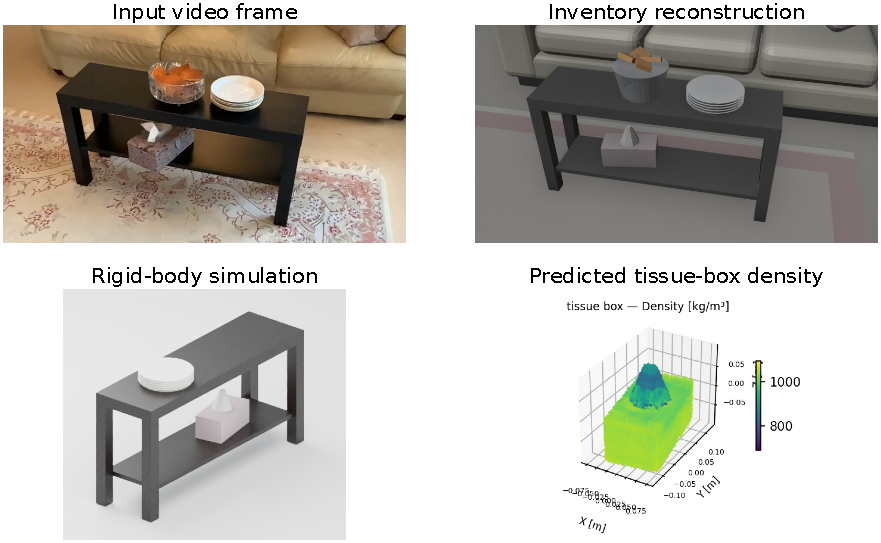
\includegraphics[width=0.93\linewidth]{figures/ca1m-coffee-physics.pdf}
\caption{From video to a physical test. The matched camera views (top) show
the plates on the tabletop and the tissue box on the shelf below. The simulation
uses those recovered meshes (bottom left). The predicted density field
(bottom right, kg/m$^3$) fills the solid tissue-box mesh, contributing to its
high estimated mass.}
\label{fig:physics}
\end{figure}

The tissue box passed the rest test, yet its estimated mass was 3.13\,kg.
Agent review flagged the mismatch between this estimate and the object's
hollow construction. The mesh occupied the equivalent of 3.08 liters of solid
material at near-water density. This explains how a stable simulation can
inherit a physically implausible mass. We lack measured masses and trajectories
for these objects, so the pilot establishes sensitivity to modeling choices.


\section{Discussion}
An agent can only repair an object's placement if it has first given that
object a separate identity. Explicit instructions addressed this omission in
each room. Detector crops helped locate additional targets, but the smaller
gain under box overlap shows that a plausible center and size can still hide a
placement error. The generation variants also depended on accurate localization.

The controller comparison exposes a trade-off in handling failures. An agent
can reconsider an individual edit, but it also spends tokens monitoring work
between edits. Python can wait for a build at no model-token cost, but a
dependency in its plan can prevent useful work after an upstream failure.
One run per controller establishes neither run-to-run cost variability nor
cost at equal quality. The CA-1M comparison covers three rooms and one seed.
Box recall omits surplus objects, category errors and fine shape. The physics
pilot needs measured object properties to establish accuracy.

\section{Conclusion}
On FloorPlan209, agent supervision achieved the highest placement recall
and carried the largest token cost. Python scheduling retained the
fitted-scale gain on small objects at 72\% lower estimated token cost than
AHA-driven, while losing five correct placements across all sizes.
Whether either controller can deliver the same quality more cheaply across
rooms remains open.
\label{main-text-end}
\clearpage
\bibliographystyle{plain}
\bibliography{references}
\end{document}
